\documentclass[tikz,border=5pt]{standalone}

\usepackage{xcolor}
\usepackage{pgfplots}
\pgfplotsset{compat=1.18}

% ---- Colors ----
\definecolor{gridgray}{RGB}{180,180,180}
\definecolor{impred}{RGB}{215,40,40}
\definecolor{synblue}{RGB}{60,110,230}
\definecolor{snipgreen}{RGB}{60,190,90}

% ---- Global styles (optional but helpful) ----
\pgfplotsset{
  myaxis/.style={
    width=12cm, height=5.2cm,
    xmin=0, xmax=7,
    ymin=55, ymax=90,
    axis lines=box,
    axis line style={black, line width=0.8pt},
    enlargelimits=false,
    xtick={0,1,2,3,4,5,6,7},
    ytick={55,60,65,70,75,80,85,90},
    ymajorgrids=true,
    xmajorgrids=false,
    grid style={gridgray, dashed},
    tick style={black},
    tick align=outside,
    label style={font=\small},
    ticklabel style={font=\small},
    legend cell align=left,
    legend columns=2,
    legend style={
      draw=black, fill=white, fill opacity=1,
      line width=0.6pt,
      font=\small,
      at={(axis cs:2.2,69)}, anchor=south west
    },
    xlabel={Time to obtain the sparse trainable network (hrs)},
    ylabel={Test accuracy (\%)}
  },
  styleIMP/.style={
    only marks, mark=triangle*, mark size=2.8pt,
    line width=0.8pt, draw=impred, fill=impred
  },
  styleSynFlow/.style={
    only marks, mark=o, mark size=3.2pt,
    line width=1.0pt, draw=synblue, fill=white
  },
  styleSNIP/.style={
    only marks, mark=diamond*, mark size=3.0pt,
    line width=0.8pt, draw=snipgreen, fill=snipgreen
  }
}

\begin{document}
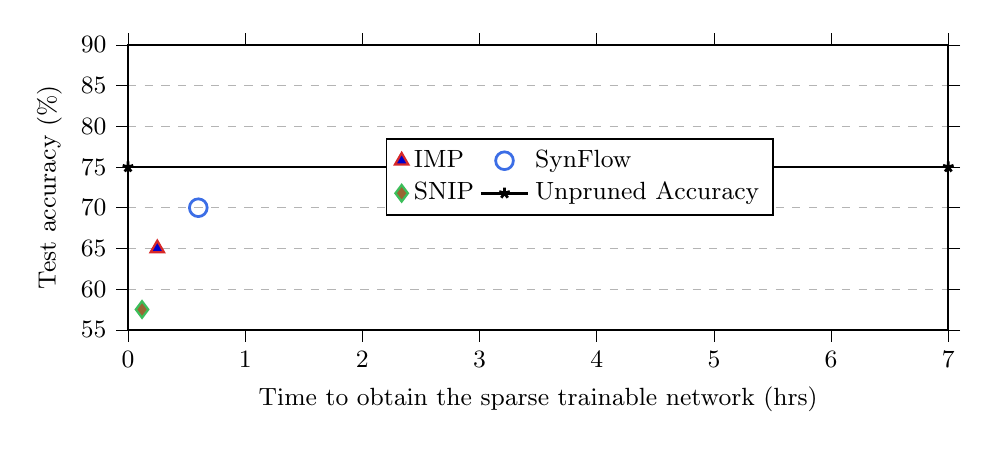
\begin{tikzpicture}
  \begin{axis}[myaxis]

    % IMP (red triangle)
    \addplot+[styleIMP] coordinates {(0.25,65)};
    \addlegendentry{IMP}

    % SynFlow (blue open circle)
    \addplot+[styleSynFlow] coordinates {(0.60,70)};
    \addlegendentry{SynFlow}

    % SNIP (green filled diamond)
    \addplot+[styleSNIP] coordinates {(0.12,57.5)};
    \addlegendentry{SNIP}

    % Unpruned Accuracy (horizontal black line)
    \addplot+[domain=0:7, samples=2, black, line width=1.0pt] {75};
    \addlegendentry{Unpruned Accuracy}

  \end{axis}
\end{tikzpicture}
\end{document}